\documentclass[12pt]{article}

% Basic packages
\usepackage{geometry}
\usepackage{amsfonts}
\usepackage{amsmath}
\usepackage{amssymb}
\usepackage{graphicx}
\usepackage[small,bf,center]{caption}
\usepackage{subfig}
\usepackage{setspace}
\usepackage{float}
\usepackage[autostyle]{csquotes}

% Packages for automated tables
\usepackage{booktabs}
\usepackage{tabularx}
\usepackage{standalone}
\usepackage{pdflscape}

\onehalfspacing
\textwidth=6.0in
\textheight=8.5in
\begin{document}

\title{My Paper}
\author{Julian Reif\thanks{University of Illinois and NBER.}}
\maketitle

\begin{abstract}
\noindent 
This paper provides an example of a document with tables and figures that were automated using Stata.
\end{abstract}

\clearpage

\section{Summary}

This example paper includes tables and figures that were created using Stata and outputted into the \textbf{/analysis/results} project folder. Copy the contents of that folder to \textbf{/paper} to update the tables and figures in this document.

Table \ref{tab:my_summary_stats} reports summary statistics for Stata's \textbf{auto.dta} dataset.%
%
\footnote{Type \textbf{sysuse auto, clear} at the Stata prompt to load this dataset.}
%
The average price of automobiles in this dataset is \$6,165. The price distribution, iillustrated in Figure \ref{fig:price_histogram}, is skewed right.

I estimate the association between automobile prices and fuel efficiency using the following linear model:
\begin{align}
PRICE_i&=\alpha + \beta X_i + \varepsilon \label{eqn:model} 
\end{align}
The outcome variable, $PRICE_i$, is the price of automobile $i$. The parameter of interest is $\beta$, a vector of coefficients. In my first specification (``spec 1''), the vector $X_i$ includes miles per gallon. The second specification (``spec 2'') also includes the car's weight. I estimate this model using ordinary least squares and report standard errors that are robust to heteroskedasticity. The analysis is performed first using Stata, and then repeated using R.

Table \ref{tab:my_regressions} reports my Stata estimates, separately for domestic and foreign cars. Column (1) reports that an increase in fuel efficiency of 1 mile per gallon is associated with a \$329 reduction in the price of domestic automobiles. Column (2) shows that this association becomes positive and insignificant when I also include weight as a regressor. Columns (3) and (4) show that these associations are similar for foreign automobiles. 

Table \ref{tab:my_regressions_with_r} compares these Stata estimates to estimates from R. Panel A reproduces the Stata estimates that were presented in Table \ref{tab:my_regressions}.  Panel B of Table \ref{tab:my_regressions_with_r} reports estimates when I repeat this analysis in R using the \textbf{lm\_robust} command from the \textit{estimatr} package. The point estimates and the standard errors are identical across both software packages.

\clearpage
\section{Figures and Tables}


%%%
% Figure: Price histogram
%%%
\begin{figure}[ht]
\caption{Automobile prices}\label{fig:price_histogram}
\begin{center}
{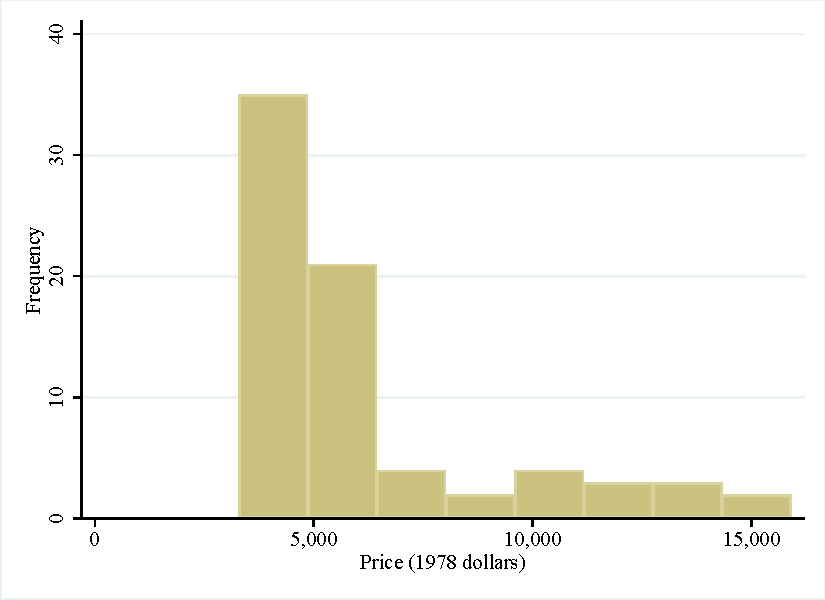
\includegraphics[width=1\textwidth]{./figures/price_histogram.pdf}}
\end{center}
\footnotesize {Notes: Data were obtained from Stata's built-in auto dataset.}
\end{figure}
\clearpage

%%%
% Tables
%%%

\documentclass{article}
\usepackage{booktabs}
\usepackage{tabularx}
\usepackage[margin=1in]{geometry}
\begin{document}

\begin{table}[tbp] \centering
\newcolumntype{C}{>{\centering\arraybackslash}X}

\caption{Summary statistics}
\label{tab:my_summary_stats}
\begin{tabularx}{\linewidth}{lCCCCC}

\toprule
{}&{Mean}&{Stdev.}&{Min}&{Max}&{Count} \tabularnewline
\midrule \addlinespace[\belowrulesep]
Weight (pounds)&3,019&777&1,760&4,840&74 \tabularnewline
Miles per gallon&21.3&5.79&12&41&74 \tabularnewline
Price (1978 dollars)&6,165&2,949&3,291&15,906&74 \tabularnewline
\bottomrule \addlinespace[\belowrulesep]

\end{tabularx}
\begin{flushleft}
\footnotesize Notes: Count reports the number of non-missing values for the variable.
\end{flushleft}
\end{table}
\end{document}

\documentclass{article}
\usepackage{booktabs}
\usepackage{tabularx}
\usepackage[margin=1in]{geometry}
\begin{document}

\begin{table}[tbp] \centering
\newcolumntype{C}{>{\centering\arraybackslash}X}

\caption{Association between automobile price and fuel efficiency}
\label{tab:my_regressions}
\begin{tabularx}{\linewidth}{lCCCC}

\toprule
&{(1)}&{(2)}&{(3)}&{(4)} \tabularnewline \midrule
& \multicolumn{2}{c}{Domestic cars} & \multicolumn{2}{c}{Foreign cars}  \tabularnewline \cmidrule(lr){2-3} \cmidrule(lr){4-5} \tabularnewline
{}&{Spec 1}&{Spec 2}&{Spec 1}&{Spec 2} \tabularnewline
\midrule \addlinespace[\belowrulesep]
Miles per gallon&--329***&238&--250**&--19.8 \tabularnewline
&(81.2)&(203)&(88.2)&(51.7) \tabularnewline
Weight (pounds)&&4.42***&&5.16*** \tabularnewline
&&(1.34)&&(0.770) \tabularnewline
\midrule N&52&52&22&22 \tabularnewline
\(R^2\)&0.254&0.483&0.399&0.785 \tabularnewline
\bottomrule \addlinespace[\belowrulesep]

\end{tabularx}
\begin{flushleft}
\footnotesize Notes: Outcome variable is price (1978 dollars). Columns (1) and (2) report estimates of \(\beta\) from equation (\ref{eqn:model}) for domestic automobiles. Columns (3) and (4) report estimates for foreign automobiles. Robust standard errors are reported in parentheses. A */**/*** indicates significance at the 10/5/1\% levels.
\end{flushleft}
\end{table}
\end{document}

\documentclass{article}
\usepackage{booktabs}
\usepackage{tabularx}
\usepackage[margin=1in]{geometry}
\begin{document}

\begin{table}[tbp] \centering
\newcolumntype{C}{>{\centering\arraybackslash}X}

\caption{Association between automobile price and fuel efficiency, Stata and R}
\label{tab:my_regressions_with_r}
\begin{tabularx}{\linewidth}{lCCCC}

\toprule
&{(1)}&{(2)}&{(3)}&{(4)} \tabularnewline \midrule
& \multicolumn{2}{c}{Domestic cars} & \multicolumn{2}{c}{Foreign cars}  \tabularnewline \cmidrule(lr){2-3} \cmidrule(lr){4-5} \tabularnewline
{}&{Spec 1}&{Spec 2}&{Spec 1}&{Spec 2} \tabularnewline
\midrule \addlinespace[\belowrulesep]
\textbf{A. Stata output (regress)}&&&& \tabularnewline
\midrule Miles per gallon&--329***&238&--250**&--19.8 \tabularnewline
&(81.2)&(203)&(88.2)&(51.7) \tabularnewline
Weight (pounds)&&4.42***&&5.16*** \tabularnewline
&&(1.34)&&(0.770) \tabularnewline
\textbf{B. R output (lm\_robust)}&&&& \tabularnewline
\midrule Miles per gallon&--329***&238&--250**&--19.8 \tabularnewline
&(81.2)&(203)&(88.2)&(51.7) \tabularnewline
Weight (pounds)&&4.42***&&5.16*** \tabularnewline
&&(1.34)&&(0.770) \tabularnewline
\bottomrule \addlinespace[\belowrulesep]

\end{tabularx}
\begin{flushleft}
\footnotesize Notes: Outcome variable is price (1978 dollars). Columns (1) and (2) report estimates of \(\beta\) from equation (\ref{eqn:model}) for domestic automobiles. Columns (3) and (4) report estimates for foreign automobiles. Robust standard errors are reported in parentheses. A */**/*** indicates significance at the 10/5/1\% levels.
\end{flushleft}
\end{table}
\end{document}


\end{document}